\documentclass{article}

\usepackage{arxiv}

\usepackage[utf8]{inputenc} % allow utf-8 input
\usepackage[T1]{fontenc}    % use 8-bit T1 fonts
\usepackage{hyperref}       % hyperlinks
\usepackage{url}            % simple URL typesettingf
\usepackage{booktabs}       % professional-quality tables
\usepackage{amsfonts}       % blackboard math symbols
\usepackage{nicefrac}       % compact symbols for 1/2, etc.
\usepackage{microtype}      % microtypography
\usepackage{lipsum}
\usepackage{graphicx}
\usepackage{tabularx}
\usepackage{wrapfig}

\usepackage[export]{adjustbox}

\usepackage{xcolor}         % http://ctan.org/pkg/xcolor

\hypersetup{
  colorlinks=true,
  linkcolor=blue!50!red,
  urlcolor=green!70!black
}

\title{A rp2040-based ultrasound pulse-echo acquisition device}

\author{
  Luc Jonveaux\thanks{More on the website \url{http://un0rick.cc}. This paper has its on Zenodo DOI  \href{http://doi.org/10.5281/zenodo.5792252}{10.5281/zenodo.5792252} } \\
  Tinkerer, Milly le Meugon, France\\
  \texttt{contact@un0rick.cc} \\
}


\begin{document}
\maketitle

\begin{abstract}
After a couple of iterations for single-element ultrasound pulse-echo devices, the pic0rick choses simplicity to reach a modular design, allowing for bipolar pulser, fast acquisition and relatively simple, barebone design. No FPGA, no BGA, plain old raspberry pico.

\end{abstract}

\keywords{arduino \and  open-source \and ultrasound \and single element \and pulse echo \and hardware \and rp2040 \and lowtech  }

\emph{ This PDF is also a ZIP that contains the sources to the hardware and some data too, don't hesitate to have a look. Just rename the file from .PDF to .ZIP and you're ready to go }.



%                .-') _  .-') _   _  .-')               
%               ( OO ) )(  OO) ) ( \( -O )              
%    ,-.-') ,--./ ,--,' /     '._ ,------.  .-'),-----. 
%    |  |OO)|   \ |  |\ |'--...__)|   /`. '( OO'  .-.  '
%    |  |  \|    \|  | )'--.  .--'|  /  | |/   |  | |  |
%    |  |(_/|  .     |/    |  |   |  |_.' |\_) |  |\|  |
%   ,|  |_.'|  |\    |     |  |   |  .  '.'  \ |  | |  |
%  (_|  |   |  | \   |     |  |   |  |\  \    `'  '-'  '
%    `--'   `--'  `--'     `--'   `--' '--'     `-----' 



%         _        ______       _       _     
%        (_)      / __   |     (_)     | |    
%   ____  _  ____| | //| | ____ _  ____| |  _ 
%  |  _ \| |/ ___) |// | |/ ___) |/ ___) | / )
%  | | | | ( (___|  /__| | |   | ( (___| |< ( 
%  | ||_/|_|\____)\_____/|_|   |_|\____)_| \_)
%  |_|                                        


\section{Overview}

The pic0rick is a very central board for an ultrasound pulse-echo system. It is composed of a main board, based on the famous rp2040 and easy to solder SMD, to which a single, and a double PMOD connector can connect to addons:
\begin{itemize}
    \item The main board is equipped with a 60Msps, 10bit ADC. Front end is protected against high-voltage pulses, and features a proven time-gain compensation system consisting in a AD8331(55.5dB) with a controlling (MCP4812) SPI DAC. PCB is 4 layers, single face - with only large SMD passives, and no BGA.
    \item The single PMOD connector can plug to the Pulser board, which can be equipped with a simple +-25V high-voltage (HV) generation board. Together, they generate the pulse on behalf of the pic0rick main board. The setup can generate three-level pulses ( with a pair of MD1210 + TC6320 ). HV board can be swapped easily.
    \item The double PMOD connector can be used for virtually anything. The current code allows for a VGA to be connected, which displays acquisitions from the board. There is also a 8 MB PSRAM module for more RAM.
\end{itemize}
The current system uses both PIOs (one for the acquisition, the other for the VGA) which leaves the other resources of the rp2040 relatively free to use for your own priorities.

\begin{figure}[htp!]
  \centering
  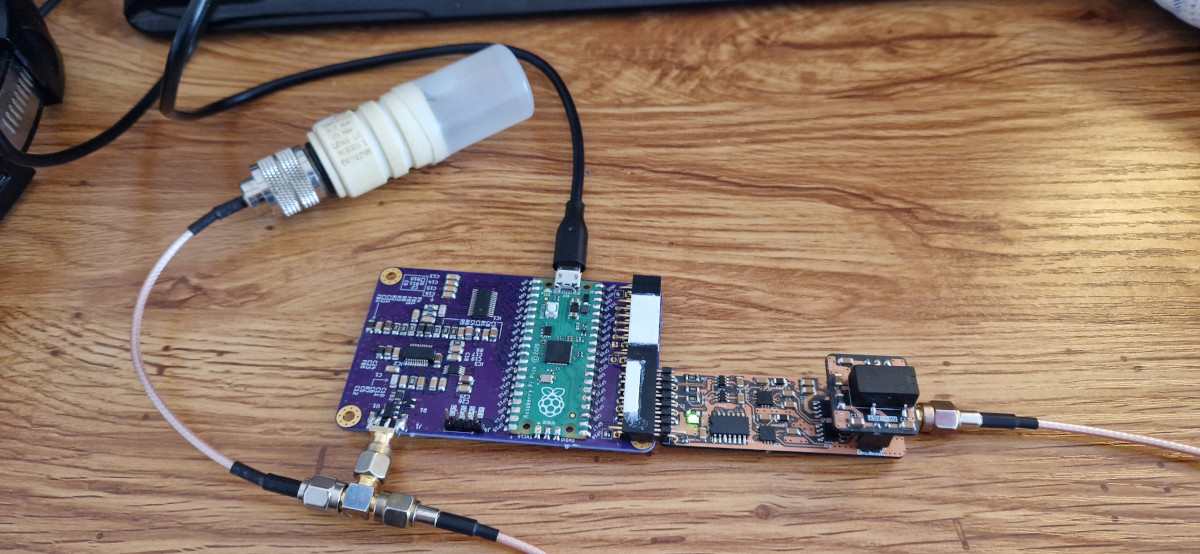
\includegraphics[width=.45\textwidth]{images/20240406_153634_s.jpg}\hfill
  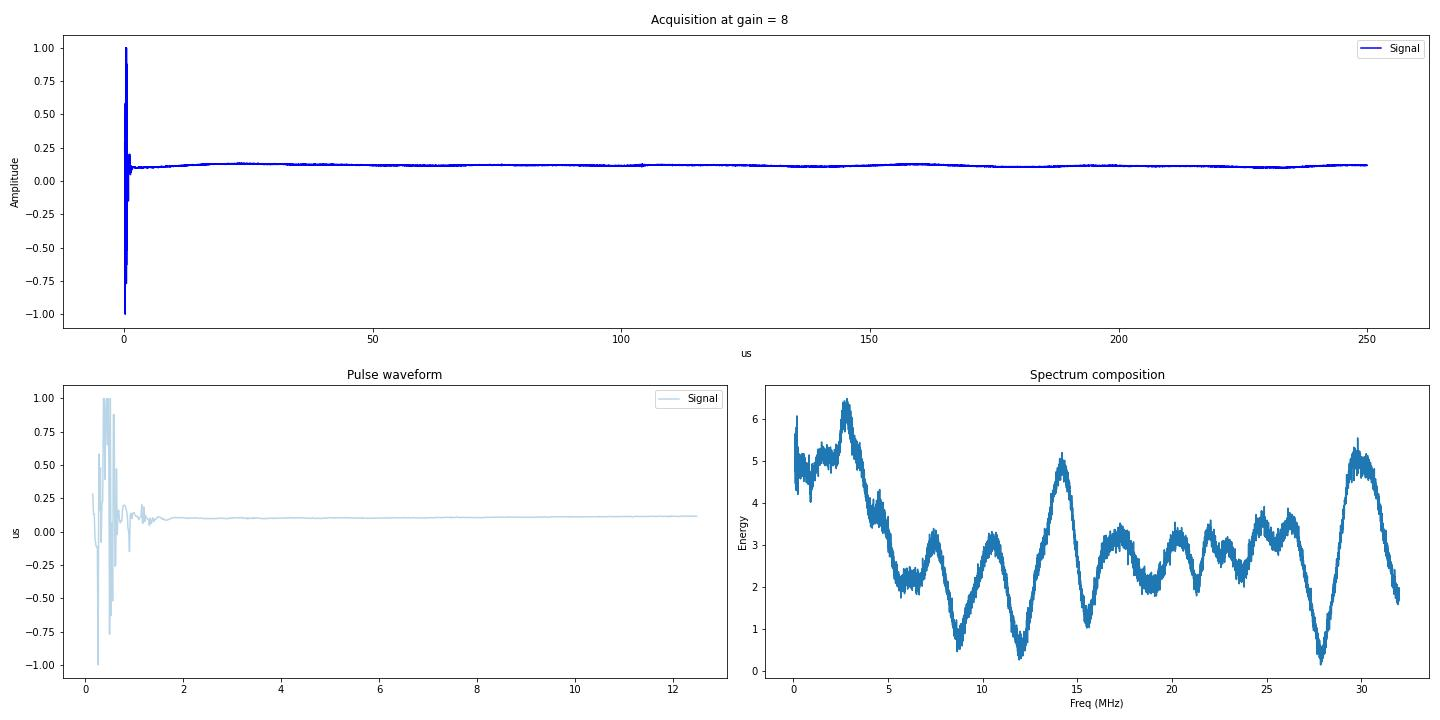
\includegraphics[width=.45\textwidth]{images/pic0gain_at_8.jpg} 
  \caption{Setup of the boards (main, pulser, hv) and resulting acquisition. VGA PMOD not connected.} 
  \label{fig:desc}
\end{figure}

\section{Where to find the latest sources} 
 

The latest sources of the hardware as well as software are available at \url{https://github.com/kelu124/pic0rick/}. However, this PDF also doubles as an archive (you can rename the .pdf as a .zip, and you'll see), and contains, in short: a set of gerbers and BOM, and some documentation. There may be some other stuff there, but I forgot what I put there. Published documents include:

\begin{itemize}
    \item KiCad design files for the main board
    \item KiCad design files for the pulser + hv boards
    \item rp2040 firmware for the microcontroller.
\end{itemize}





 \section{Next steps}

Plenty to do on the next steps. The current shopping list (non-exhaustive) may include:


\begin{itemize}
    \item Hardware: Slight tweaks on the main board to allow more space for the PMODs, include OSHWA certfication number, ..
   \item Firmware: Tie the pulses to the PIO code so that pulses strictly cohappen with the acquisition start 
\end{itemize}


\section{Links to go further}

\begin{itemize}
\item Come and chat : \href{https://join.slack.com/usdevkit/shared_invite/MTkxODU5MjU0NjI1LTE0OTY1ODgxMDEtMmYyZTliZDBlZA}{join the Slack channel} 
\item The full GitHub repository for \href{https://github.com/kelu124/pic0rick}{the pic0rick "motherboard"}.
\item The board’s \href{https://www.tindie.com/stores/kelu124/}{Tindie shop} to get it
\item Check out \href{http://doi.org/10.5334/joh.28}{my previous work} on the topic of ultrasound modules \cite{review} and its \href{http://doi.org/10.5281/zenodo.377054}{dataset on Zenodo}. More to come!
\end{itemize}

\section*{License}


%
%                                                                      
%  ____ ______   ____   ____     __________  __ _________  ____  ____  
% /  _ \\____ \_/ __ \ /    \   /  ___/  _ \|  |  \_  __ _/ ____/ __ \ 
%(  <_> |  |_> \  ___/|   |  \  \___ (  <_> |  |  /|  | \\  \__\  ___/ 
% \____/|   __/ \___  |___|  / /____  \____/|____/ |__|   \___  \___  >
%       |__|        \/     \/       \/                        \/    \/ 
%

This work is based on previous projects, the un0rick, lit3rick and the echOmods projects. The pic0rick project and its boards are open hardware and software, developed with open-source elements.

Copyright Luc Jonveaux / kelu124 (kelu124@gmail.com) 2024

\begin{itemize}
\item The hardware is licensed under TAPR Open Hardware License (www.tapr.org/OHL)
\item The software components are free software: you can redistribute it and/or modify it under the terms of the GNU General Public License as published by the Free Software Foundation, either version 3 of the License, or (at your option) any later version.
\item The documentation is licensed under a Creative Commons Attribution-ShareAlike 3.0 Unported License.
\end{itemize}



\bibliographystyle{unsrt}  
%\bibliography{references}  %%% Remove comment to use the external .bib file (using bibtex).
%%% and comment out the ``thebibliography'' section.


%%% Comment out this section when you \bibliography{references} is enabled.
\begin{thebibliography}{1}

  \bibitem{kelu124}
  Luc Jonveaux 2017.
  \newblock  Arduino-like development kit for single-element ultrasound imaging. 
  \newblock In {\em  Journal of Open Hardware, 1(1), p.3}. DOI: \href{http://doi.org/10.5334/joh.2}{10.5334/joh.2}
  
  \bibitem{un0rick}
  Luc Jonveaux 2019.
  \newblock  un0rick : open-source fpga board for single element ultrasound imaging
  \newblock On {\em  Zenodo}. DOI: \href{http://doi.org/10.5281/zenodo.3364559}{10.5281/zenodo.3364559}
  
  \bibitem{lit3rick}
  Luc Jonveaux 2021.
  \newblock lit3rick: an up5k ultrasound pulse-echo device %%@todo change title
  \newblock On {\em  Zenodo}. DOI: \href{http://doi.org/10.5281/zenodo.5792245}{10.5281/zenodo.5792245}
  
%% @TODO
    \bibitem{review}
  Luc Jonveaux, Carla Schloh, William Meng, Jorge Arija, Jean Rintoul 2024.
  \newblock Review of Current Simple Ultrasound Hardware Considerations, Designs, and Processing Opportunities
  \newblock On {\em  Journal of Open Hardware (JOH) }. DOI: \href{http://doi.org/10.5334/joh.28}{10.5334/joh.28}
%% @TODO
      \bibitem{max14866}
  Luc Jonveaux 2021.
  \newblock An opensource max14866 development board %%@todo change title
  \newblock On {\em  Zenodo}. DOI: \href{http://doi.org/10.5281/zenodo.5792252}{10.5281/zenodo.5792252}
  
\end{thebibliography}




\end{document}


% Subertley     
%                                             
%  .__  .__  __ ________       .__        __    
%  |  | |__|/  |\_____  \______|__| ____ |  | __
%  |  | |  \   __\_(__  <_  __ \  |/ ___\|  |/ /
%  |  |_|  ||  | /       \  | \/  \  \___|    < 
%  |____/__||__|/______  /__|  |__|\___  >__|_ \
%                      \/              \/     \/
%  